% =============================================================================
% MAM Orientation BootCamp — Probability and Statistics Foundations
% Part 1: Random Variables and Distributions  (50 min)
% =============================================================================
% Technical content: Wooldridge (2016), Appendix B-1
% Figures:           scripts/R/part1_figures.R  ->  output/figures/p1_*.pdf
% Compile:  cd drafts/slides
%           TEXINPUTS=../latex_files: xelatex part1_random_variables.tex
%           BIBINPUTS=../latex_files: bibtex part1_random_variables
%           (then two more xelatex passes)
% =============================================================================
\documentclass[9pt,english,aspectratio=169]{beamer}
\input{../latex_files/header_slides}

\bibliographystyle{../latex_files/aea}

\graphicspath{{../../output/figures/}}

% ---------- Title ----------
\title{\textbf{Random Variables and Distributions}}
\subtitle{Probability and Statistics Foundations --- Part 1}
\author{Instructor: Tudor Schlanger}
\date{Master's in Asset Management \\ Yale School of Management}

\begin{document}

% =============================================================================
% Title
% =============================================================================
\begin{frame}
  \titlepage
\end{frame}

\begin{frame}{Objectives for this session}
  \large
  \begin{enumerate}
    \item Expose you to ideas and terminology \\[1em]
    \item Teach you how we map the real world to math objects \\[1em]
    \item Teach you how to interpret math objects using real world examples
  \end{enumerate}
  
\end{frame}

\begin{frame}{Random processes}

  \begin{columns}[T]
    \begin{column}{0.49\textwidth}
      \includegraphics[width=\textwidth]{p1_returns_a_blind.pdf}
    \end{column}
    \begin{column}{0.49\textwidth}
      \includegraphics[width=\textwidth]{p1_returns_b_blind.pdf}
    \end{column}
  \end{columns}

  \pause 
  \vspace{0.5em}
  \begin{questionbox}
    Which one is actual return, which one is simulated?
  \end{questionbox}

\end{frame}

\begin{frame}{Random processes}

  \begin{columns}[T]
    \begin{column}{0.49\textwidth}
      \includegraphics[width=\textwidth]{p1_returns_a_revealed.pdf}
    \end{column}
    \begin{column}{0.49\textwidth}
      \includegraphics[width=\textwidth]{p1_returns_b_revealed.pdf}
    \end{column}
  \end{columns}

  \vspace{0.5em}
  \begin{questionbox}
    Which one is actual return, which one is simulated?
  \end{questionbox}

\end{frame}

\begin{frame}{Random processes}

  \begin{columns}[T]
    \begin{column}{0.49\textwidth}
      \includegraphics[width=\textwidth]{p1_returns_a_revealed.pdf}
    \end{column}
    \begin{column}{0.49\textwidth}
      \includegraphics[width=\textwidth]{p1_dist_normal.pdf}

      % \vspace{0.35em}
      % \includegraphics[width=\textwidth]{p1_dist_kde.pdf}
    \end{column}
  \end{columns}

\end{frame}


\begin{frame}{Outline}

  \large 
  \begin{enumerate}
    \item[\textbf{1.}] Random variables and distributions \\
          {\small\textcolor{DarkGray}{How do we describe an uncertain outcome mathematically?}}
          \vspace{0.5em}
    \item[\textbf{2.}] Population parameters and moments \\
          {\small\textcolor{DarkGray}{If we know the distribution, which summary numbers matter?}}
          \vspace{0.5em}
    \item[\textbf{3.}] Statistical inference \\
          {\small\textcolor{DarkGray}{If we \emph{don't} know the distribution, how do we learn it from data?}}
  \end{enumerate}

\end{frame}


\begin{frame}{Outline}


  \large
  \begin{enumerate}
    \item[\textbf{1.}] \textbf{Random variables and distributions} \\
          {\small\textcolor{DarkGray}{How do we describe an uncertain outcome mathematically?}}
          \vspace{0.5em}
    \item[\textbf{2.}] Population parameters and moments \\
          {\small\textcolor{DarkGray}{If we know the distribution, which summary numbers matter?}}
          \vspace{0.5em}
    \item[\textbf{3.}] Statistical inference \\
          {\small\textcolor{DarkGray}{If we \emph{don't} know the distribution, how do we learn it from data?}}
  \end{enumerate}

\end{frame}

\begin{frame}{Start With a Data Generating Process}

  \begin{columns}[T]
    \begin{column}{0.5\textwidth}
      \begin{definitionbox}[Data generating process (DGP)]
        Any mechanism that could, in principle, be \textbf{run
        indefinitely} and has a well-defined set of possible \textbf{outcomes}.
      \end{definitionbox}

      \vspace{0.8em}
      Before the DGP runs we do not know the outcome. Afterwards we do.
    \end{column}
    \pause 
    \begin{column}{0.48\textwidth}
      \vspace{0.8em}
      Example 1: 
      \begin{itemize}
        \item \textbf{DGP:} Flip a coin once
        \item \textbf{Outcome:} Heads
      \end{itemize}
      \vspace{1em}
      Example 2: 
      \begin{itemize}
        \item \textbf{DGP:} Stock market trades for 1 day
        \item \textbf{Outcome:} Market price rises
      \end{itemize}     
    \end{column}
  \end{columns}

\end{frame}

\begin{frame}{Random Variables: From Outcomes to Numbers}

  \begin{insightbox}
      A data generating process produces \textbf{outcomes}. \\
      A random variable turns each outcome into a \textbf{number}.
  \end{insightbox}

  \pause
  \vspace{0.3em}
  \begin{definitionbox}[Random variable]
    A random variable is a \textbf{function}. 
    $$X: \Omega \rightarrow \R$$
  \end{definitionbox}
  \pause 
  \vspace{0.5em}
  \begin{center}
  \begin{tikzpicture}[
      outcome/.style={draw=DarkGray, fill=softbg, rounded corners=2pt,
                      minimum width=2.5cm, minimum height=0.62cm, font=\small},
      xarrow/.style={-{Stealth[length=2mm]}, blue, thick}
    ]

    % --- Outcome space: one row of possible outcomes ---
    \node[font=\small\bfseries, anchor=west] at (-0.9, 1.75)
      {Outcomes of the DGP ($\Omega$)};
    \node[outcome] (down) at (1.6, 1.15) {Market falls};
    \node[outcome] (flat) at (5.0, 1.15) {Market flat};
    \node[outcome] (up)   at (8.4, 1.15) {Market rises};

    \pause

    % --- The mapping: straight down, no crossings ---
    \foreach \n in {down, flat, up}{
      \draw[xarrow] (\n.south) -- ++(0, -0.62);
    }
    \node[blue, font=\small\bfseries, anchor=west] at (5.25, 0.55) {$X$};

    \pause

    % --- Number line ---
    \draw[thick, black] (0.1, 0) -- (9.9, 0);
    \foreach \x/\lab in {1.6/-1, 5.0/0, 8.4/1}{
      \draw[thick] (\x, 0.13) -- (\x, -0.13);
      \node[font=\small, below=2pt] at (\x, -0.13) {\lab};
    }
    \node[font=\small\bfseries, anchor=west] at (-0.9, -0.75) {The real line ($\R$)};

  \end{tikzpicture}
  \end{center}


\end{frame}

% \begin{frame}{Definition}

%   \begin{columns}[T]
%     \begin{column}{0.56\textwidth}
%       \begin{definitionbox}[Random Variable]
%         A variable that takes on \textbf{numerical values}, with the value
%         determined by the outcome of the DGP.
%       \end{definitionbox}
%       \pause

%       \vspace{0.8em}
%       Note what this rules out. A random variable is \emph{not}:
%       \begin{itemize}
%         \item ``the market'' \hfill {\small\textcolor{DarkGray}{(not a number)}}
%               \vspace{0.25em}
%         \item ``rises or falls'' \hfill {\small\textcolor{DarkGray}{(not a number --- yet)}}
%       \end{itemize}
%       \pause

%       \vspace{0.6em}
%       Qualitative events are fine, as long as we \textbf{assign numbers} to
%       them --- as we just did with $-1, 0, 1$.
%     \end{column}
%     \begin{column}{0.40\textwidth}
%       \vspace{1.5em}
%       \begin{methodbox}
%         The number assignment is a \textbf{choice}. We could have used
%         $0$ and $1$, or the actual percentage return. Different choices answer
%         different questions.
%       \end{methodbox}
%     \end{column}
%   \end{columns}

%   \vspace{0.5em}

% \end{frame}


\begin{frame}{Random Variables in Finance}

  \vspace{0.3em}
  \centering
  \renewcommand{\arraystretch}{1.45}
  \begin{tabular}{@{} l l l @{}}
    \toprule
    \textbf{Period}     & \textbf{DGP}              & \textbf{Values  $X$ can take} \\
    \midrule
    One trading day     & Did the market rise?          & $\{ 0, 1 \}$ \\
    Two trading days    & Number of up days             & $\{0, 1, 2\}$ \\
    One week            & Number of trades executed     & $\{0, 1, 2, \ldots\}$ \\
    One month           & \% Return on the S\&P 500     & $[-100; \infty)$ \\
    \bottomrule
  \end{tabular}
  \pause

  \vspace{1.2em}
  \begin{insightbox}
    Look at the last column. Some lists are \textbf{discrete}, some are \textbf{continuous}. 
  \end{insightbox}

\end{frame}


\begin{frame}{Two Kinds of Random Variables}

  % Built in four steps: each support first, then the distribution that sits
  % directly underneath it. The distributions share the supports' x coordinates,
  % so every bar stands under its own value and the density under its range.
  \vspace{0.3em}
  \begin{center}
  \begin{tikzpicture}[font=\small,
      spinearrow/.style={-{Stealth[length=2mm]}, blue, thick}]

    % Reserve the full extent from the start -- including the spine column on
    % the left, whose bottom label only arrives on overlay 3 -- so nothing
    % shifts as the later overlays add content.
    \path (-2.05, 2.8) (11.8, -2.9);

    % --- Spine: what each row of the picture is ---
    % Omega (outcomes) -> X (the values on the line) -> P(X = x) (the bars).
    % Column titles sit above the spine, so each column reads title, then
    % example, then values, then distribution.
    \node[font=\small, anchor=center] at (-1.25, 1.85) {$\Omega$};
    \draw[spinearrow] (-1.25, 1.57) -- (-1.25, 0.95);
    \node[font=\small, anchor=center] at (-1.25, 0.7) {$X$};

    % --- Discrete: the support ---
    % Centred on the discrete number line below (which runs 0 to 5.2).
    \node[font=\small\bfseries, anchor=center] at (2.6, 2.55) {\textbf{DISCRETE RANDOM VARIABLE}};
    \node[font=\small, anchor=west] at (-0.4, 1.85)
      {\textbf{Example:} number of trades executed};
    \draw[thick, black] (0, 0.7) -- (5.2, 0.7);
    \foreach \x in {0.4, 1.4, 2.4, 3.4, 4.4}{
      \filldraw[blue] (\x, 0.7) circle (2.6pt);
    }
    \foreach \x/\lab in {0.4/0, 1.4/1, 2.4/2, 3.4/3, 4.4/4}{
      \node[below=3pt, font=\scriptsize] at (\x, 0.7) {\lab};
    }
    \node[font=\scriptsize, anchor=west, DarkGray] at (0, 0.05)
      {gaps in between --- nothing can land there};

    \pause

    % --- Continuous: the support ---
    % This half sits 0.8 left of where it used to, to free the spine column.
    % Centred on the continuous number line below (which runs 6.6 to 11.8).
    \node[font=\small\bfseries, anchor=center] at (9.2, 2.55) {\textbf{CONTINUOUS RANDOM VARIABLE}};
    \node[font=\small, anchor=west] at (6.2, 1.85)
      {\textbf{Example:} \% return on the S\&P 500};
    \draw[thick, black] (6.6, 0.7) -- (11.8, 0.7);
    \draw[line width=3.5pt, orange, opacity=0.75] (7.1, 0.7) -- (11.3, 0.7);
    \foreach \x/\lab in {7.1/{-10\%}, 9.2/{0\%}, 11.3/{10\%}}{
      \draw[thick] (\x, 0.82) -- (\x, 0.58);
      \node[below=3pt, font=\scriptsize] at (\x, 0.7) {\lab};
    }
    \node[font=\scriptsize, anchor=west, DarkGray] at (6.6, 0.05)
      {no gaps --- every value in between is possible};

    \pause

    % --- Spine: the distribution level ---
    \draw[spinearrow] (-1.25, 0.42) -- (-1.25, -1.3);
    \node[font=\small, anchor=center] at (-1.25, -1.6) {$\Prob(X = x)$};

    % --- Discrete: its distribution, directly below the support ---
    % Bar heights are Binomial(4, 0.55) probabilities scaled by 4.0.
    \node[font=\small\bfseries, anchor=west] at (-0.4, -0.35)
      {Its distribution: a bar on each value};
    \node[font=\scriptsize, anchor=west, DarkGray] at (-0.4, -0.7)
      {height $=\Prob(X = x)$};
    \foreach \x/\barTop in {0.4/-2.24, 1.4/-1.60, 2.4/-0.93, 3.4/-1.20, 4.4/-2.03}{
      \draw[blue, line width=7pt, opacity=0.85] (\x, -2.4) -- (\x, \barTop);
    }
    \draw[thick, black] (0, -2.4) -- (5.2, -2.4);
    \node[font=\scriptsize, anchor=west, DarkGray] at (0, -2.75)
      {the five heights add to $1$};

    \pause

    % --- Continuous: its distribution, directly below the support ---
    \node[font=\small\bfseries, anchor=west] at (6.2, -0.35)
      {Its distribution: a curve over the range};
    \node[font=\scriptsize, anchor=west, DarkGray] at (6.2, -0.7)
      {area $=\Prob(a \le X \le b)$};
    \fill[orange, opacity=0.25]
      plot[domain=6.7:11.7, samples=140, smooth]
        (\x, {-2.4 + 1.47*exp(-((\x-9.2)^2)/(2*0.84*0.84))})
      -- (11.7, -2.4) -- (6.7, -2.4) -- cycle;
    \draw[orange, line width=1pt]
      plot[domain=6.7:11.7, samples=140, smooth]
        (\x, {-2.4 + 1.47*exp(-((\x-9.2)^2)/(2*0.84*0.84))});
    \draw[thick, black] (6.6, -2.4) -- (11.8, -2.4);
    \node[font=\scriptsize, anchor=west, DarkGray] at (6.6, -2.75)
      {the shaded area is $1$};

  \end{tikzpicture}
  \end{center}

\end{frame}


\begin{frame}{Notation: $X$ Versus $x$}


  \vspace{0.8em}
  \begin{columns}[T]
    \begin{column}{0.46\textwidth}
      \begin{definitionbox}[$X$ --- uppercase]
        The random variable itself \\

        e.g. ``$X$ is next month's return.''
      \end{definitionbox}
    \end{column}
    \pause
    \begin{column}{0.46\textwidth}
      \begin{definitionbox}[$x$ --- lowercase]
        A realized value. \\

        e.g. ``This month's return was $x = 2.3\%$.''
      \end{definitionbox}
    \end{column}
  \end{columns}

\end{frame}

% Superseded: these bars and this density now live directly underneath
% their supports on the "Two Kinds of Random Variables" frame above.
% \begin{frame}{Where the Probability Sits}
%
%   % Same two number lines as the previous frame, same coordinates -- the only
%   % new thing is the probability drawn on top of them.
%   \vspace{0.3em}
%   \begin{center}
%   \begin{tikzpicture}[font=\small]
%
%     % --- Discrete: a bar standing on each value ---
%     \node[font=\small\bfseries, anchor=west] at (-0.4, 3.15)
%       {\textbf{Discrete:} a bar on each value};
%     \node[font=\scriptsize, anchor=west, DarkGray] at (-0.4, 2.8)
%       {height $=\Prob(X = x)$};
%
%     % Heights are Binomial(4, 0.55) probabilities, scaled by 4.5
%     \foreach \x/\top in {0.4/0.89, 1.4/1.60, 2.4/2.35, 3.4/2.05, 4.4/1.11}{
%       \draw[blue, line width=7pt, opacity=0.85] (\x, 0.7) -- (\x, \top);
%     }
%     \draw[thick, black] (0, 0.7) -- (5.2, 0.7);
%     \foreach \x/\lab in {0.4/0, 1.4/1, 2.4/2, 3.4/3, 4.4/4}{
%       \node[below=3pt, font=\scriptsize] at (\x, 0.7) {\lab};
%     }
%     \node[font=\scriptsize, anchor=west, DarkGray] at (0, 0.05)
%       {the five heights add to $1$};
%
%     \pause
%
%     % --- Continuous: a density spread over the range ---
%     \node[font=\small\bfseries, anchor=west] at (7.0, 3.15)
%       {\textbf{Continuous:} a curve over the range};
%     \node[font=\scriptsize, anchor=west, DarkGray] at (7.0, 2.8)
%       {area $=\Prob(a \le X \le b)$};
%
%     \fill[orange, opacity=0.25]
%       plot[domain=7.5:12.5, samples=140, smooth]
%         (\x, {0.7 + 1.65*exp(-((\x-10)^2)/(2*0.84*0.84))})
%       -- (12.5, 0.7) -- (7.5, 0.7) -- cycle;
%     \draw[orange, line width=1pt]
%       plot[domain=7.5:12.5, samples=140, smooth]
%         (\x, {0.7 + 1.65*exp(-((\x-10)^2)/(2*0.84*0.84))});
%
%     \draw[thick, black] (7.4, 0.7) -- (12.6, 0.7);
%     \foreach \x/\lab in {7.9/{-10\%}, 10.0/{0\%}, 12.1/{10\%}}{
%       \draw[thick] (\x, 0.82) -- (\x, 0.58);
%       \node[below=3pt, font=\scriptsize] at (\x, 0.7) {\lab};
%     }
%     \node[font=\scriptsize, anchor=west, DarkGray] at (7.4, 0.05)
%       {the shaded area is $1$};
%
%   \end{tikzpicture}
%   \end{center}
%   \pause
%
%   \begin{insightbox}
%     Same job, two ways of carrying it: \textbf{stack} the probability on the
%     values, or \textbf{spread} it along the range.
%   \end{insightbox}
%
% \end{frame}

% The buttons jump to the appendix, where the Bernoulli, Binomial and Poisson
% detail now lives. `label=discreterv' is the target the return buttons use.
\begin{frame}[label=discreterv]{Discrete Random Variables}

  \begin{columns}[T]
    \begin{column}{0.48\textwidth}
      \begin{definitionbox}[Probability mass function (pmf)]
        You can list the values $x_1, x_2, \ldots$ \\[0.3em]
        Its distribution is described by a \\ \textbf{probability mass function}
        \[ f(x) = \Prob(X = x) \]
      \end{definitionbox}
      \vspace{0.2em}
      {\scriptsize\textcolor{DarkGray}{Some texts call this a pdf too; we say
      \textbf{pmf} for the discrete case.}}

      \vspace{0.2em}
      \onslide<2->{%
        \textbf{Distributions:} \hfill {\small\textcolor{DarkGray}{and their support}}
        \begin{itemize}\setlength{\itemsep}{0pt}
          \item \hyperlink{appbernoulli}{\beamergotobutton{Bernoulli}} \hfill {\small\textcolor{DarkGray}{$\{0, 1\}$}}
          \item \hyperlink{appbinomial}{\beamergotobutton{Binomial}} \hfill {\small\textcolor{DarkGray}{$\{0, 1, 2, \ldots, N\}$}}
          \item \hyperlink{apppoisson}{\beamergotobutton{Poisson}} \hfill {\small\textcolor{DarkGray}{$\{0, 1, 2, \ldots \}$}}
        \end{itemize}%
      }
    \end{column}
    \begin{column}{0.48\textwidth}
      % Same Binomial(4, 0.55) heights as the TikZ bars on "Two Kinds of Random
      % Variables", with the probabilities printed: both properties below can be
      % read straight off the picture.
      \includegraphics[width=\textwidth]{p1_pmf_generic.pdf}

      \vspace{0.5em}
      \onslide<3->{%
        \begin{definitionbox}[Some properties]
          \begin{enumerate}\setlength{\itemsep}{0.35em}
            \item[\textbf{1.}] $0 \leq f(x) \leq 1$ for every $x$ \\
            \item[\textbf{2.}] $\displaystyle\sum_{x} f(x) = 1$
          \end{enumerate}
        \end{definitionbox}%
      }

    \end{column}
  \end{columns}

\end{frame}

\begin{frame}{Continuous Random Variables}

  % Question and answer face each other, then the insight lands underneath both.
  % Explicit \onslide, not \pause: these box environments typeset their body
  % outside the pause scope, so a preceding \pause leaves them visible from the
  % first overlay.
  \begin{columns}[T]
    \begin{column}{0.48\textwidth}
      \begin{questionbox}
        What is the probability that next month's S\&P return is
        \textbf{exactly} $0.5\%$?
      \end{questionbox}
    \end{column}
    \begin{column}{0.48\textwidth}
      \onslide<2->{%
        \begin{answerbox}
          \textbf{Zero.}

          \vspace{0.4em}
          Not ``very small'' --- exactly zero.
        \end{answerbox}%
      }
    \end{column}
  \end{columns}

  \vspace{0.6em}
  \onslide<3->{%
    \begin{insightbox}
      The values fill a range, so \textbf{no single value carries probability}:
      $\Prob(X = x) = 0$ for any $x$.
    \end{insightbox}%
  }

  \onslide<4->{%
    \vspace{0.5em}
    Why? A probability function must add up to $1$. \\
    If $\Prob(X = x) > 0$ for uncountably many values of $x$, the total could never stay finite --- let alone equal $1$.
  }

\end{frame}

\begin{frame}{Continuous Random Variables}

  \begin{columns}[T]
    \begin{column}{0.48\textwidth}
      \begin{definitionbox}[Probability density function (pdf)]
        Probability attaches to a \textbf{range} $[a, b]$, through a \\
        \textbf{probability density function} $f(x)$: 
        \[ \Prob(a \le X \le b) = \int_a^b f(x)\,dx \]
      \end{definitionbox}


      \vspace{0.2em}
      \onslide<2->{%
        \textbf{Distributions:} \hfill {\small\textcolor{DarkGray}{and their support}}
        \begin{itemize}\setlength{\itemsep}{0pt}
          \item Normal \hfill {\small\textcolor{DarkGray}{$(-\infty, \infty)$}}
          \item Lognormal \hfill {\small\textcolor{DarkGray}{$(0, \infty)$}}
          \item Student-$t$ \hfill {\small\textcolor{DarkGray}{$(-\infty, \infty)$}}
        \end{itemize}%
      }
    \end{column}
    \begin{column}{0.48\textwidth}
      % Sized to match p1_pmf_generic.pdf on the facing discrete frame, so the
      % two slides put their picture and their properties box at the same height.
      \begin{center}
        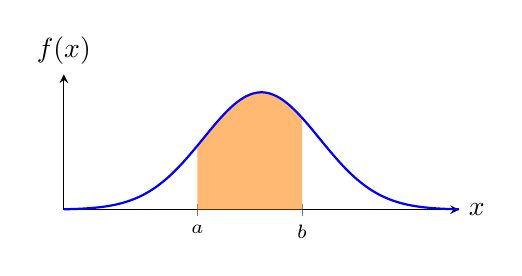
\begin{tikzpicture}
          \begin{axis}[
              width=6.6cm, height=3.3cm,
              axis lines=left,
              xtick={-1.1, 0.7}, xticklabels={$a$, $b$},
              ytick=\empty,
              xmin=-3.4, xmax=3.4, ymin=0, ymax=0.46,
              xlabel={$x$}, ylabel={$f(x)$},
              tick label style={font=\scriptsize},
              label style={font=\scriptsize},
              every axis x label/.style={at={(current axis.right of origin)},
                anchor=west},
              every axis y label/.style={at={(current axis.north west)},
                anchor=south, rotate=0},
              clip=false
            ]
            \addplot[draw=none, fill=orange, fill opacity=0.55, domain=-1.1:0.7,
                    samples=80]
              {0.3989*exp(-0.5*x^2)} \closedcycle;
            \addplot[blue, thick, domain=-3.4:3.4, samples=140]
              {0.3989*exp(-0.5*x^2)};
          \end{axis}
        \end{tikzpicture}
      \end{center}

    \end{column}
  \end{columns}

\end{frame}



\begin{frame}{Properties}

  \begin{columns}[T]
    \begin{column}{0.40\textwidth}
      \vspace{0.8em}
      \vspace{0.2em}
      \begin{definitionbox}[Some properties]
        \begin{enumerate}\setlength{\itemsep}{0.35em}
          \item[\textbf{1.}] $f(x) \geq 0$ for every $x$ \\
          \item[\textbf{2.}] $\displaystyle\int_{-\infty}^{\infty} f(x)\,dx = 1$
        \end{enumerate}
      \end{definitionbox}
      \vspace{0.2em}
      Note that $f(x)$ \textbf{can} exceed 1 --- it is a \emph{density}, not a
              probability.
    \end{column}
    \begin{column}{0.56\textwidth}
      \vspace{0.8em}
      \begin{center}
      \begin{tikzpicture}
        \begin{axis}[
            width=7.6cm, height=4.2cm,
            axis lines=left,
            xtick=\empty, ytick=\empty,
            xmin=-3.4, xmax=3.4, ymin=0, ymax=0.46,
            xlabel={$x$}, ylabel={$f(x)$},
            every axis x label/.style={at={(current axis.right of origin)},
              anchor=west},
            every axis y label/.style={at={(current axis.north west)},
              anchor=south},
            clip=false
          ]
          \addplot[draw=none, fill=skyblue, fill opacity=0.5, domain=-3.4:3.4,
                   samples=140]
            {0.3989*exp(-0.5*x^2)} \closedcycle;
          \addplot[blue, thick, domain=-3.4:3.4, samples=140]
            {0.3989*exp(-0.5*x^2)};
          \node[font=\large] at (axis cs:0, 0.16) {area $= 1$};
        \end{axis}
      \end{tikzpicture}
      \end{center}
    \end{column}
  \end{columns}

\end{frame}

\begin{frame}{Probabilities with Real Data}

  \begin{columns}[T]
    \begin{column}{0.44\textwidth}
      \vspace{0.5em}
      \begin{questionbox}
        What is the probability that the S\&P 500 has a \textbf{losing} month?
      \end{questionbox}

      \onslide<2->{%
        \vspace{0.8em}
        In symbols, we want
        \[
          \Prob(X < 0),
        \]
        which is the area under the curve --- the whole left tail.%
      }

    \end{column}
    \begin{column}{0.52\textwidth}
      % Was 1.5em: the answer box now sits full width below the columns, so the
      % frame needs the height back.
      \vspace{0.3em}
      % Bare density while the question is on screen; the shading (and the
      % printed area) arrives with the answer. Both files are drawn on the same
      % axes in part1_figures.R, so the swap does not move anything.
      \only<1-2>{\includegraphics[width=\textwidth]{p1_density_plain.pdf}}%
      \only<3->{\includegraphics[width=\textwidth]{p1_density_interval.pdf}}

      \vspace{0.2em}
      {\tiny\textcolor{lightgray}{Estimated density of real S\&P monthly returns, 1871--2026.}}
    \end{column}
  \end{columns}
      \onslide<3->{%
        \begin{answerbox}
          About \textbf{0.43}

          \vspace{0.3em}
          {\small $801$ of the $1{,}867$ months since 1871.}
        \end{answerbox}%
      }

\end{frame}

\begin{frame}{From pdf to cdf}

  \begin{columns}[T]
    \begin{column}{0.54\textwidth}
      \begin{definitionbox}[Cumulative Distribution Function (cdf)]
        For any number $x$,
        \[
          F(x) = \Prob(X \leq x)
        \]
        --- all the area to the \textbf{left} of $x$.
      \end{definitionbox}
    \end{column}
    \begin{column}{0.42\textwidth}

      \vspace{0.6em}
      \begin{enumerate}
        \item $0 \leq F(x) \leq 1$ 
              \hfill {\small\textcolor{DarkGray}{it is a probability}}
              \vspace{0.5em}
        \pause
        \item $F(x) \to 0$ far to the left. \\
               $F(x) \to 1$ far to the right.
        \pause
        \item $F$ never decreases.
              \hfill {\small\textcolor{DarkGray}{area only accumulates}}
              \vspace{0.5em}

      \end{enumerate}
    \end{column}
  \end{columns}

\end{frame}

\begin{frame}{The Same Idea, Two Pictures}

  \centering
  \includegraphics[width=0.76\textwidth]{p1_pdf_cdf_pair.pdf}
  

\end{frame}


\begin{frame}{More on cdf}

  \begin{columns}[T]
    \begin{column}{0.47\textwidth}
      \begin{methodbox}
        \textbf{Property 1 --- the right tail}
        \[
          \Prob(X > c) = 1 - F(c)
        \]
        \vspace{-0.6em}

        {\small Everything, minus what is to the left.}
      \end{methodbox}
    \end{column}

    \begin{column}{0.47\textwidth}
      \begin{methodbox}
        \textbf{Property 2 --- a middle slice}
        \[
          \Prob(a < X \leq b) = F(b) - F(a)
        \]
        \vspace{-0.6em}

        {\small Left of $b$, minus left of $a$.}
      \end{methodbox}
    \end{column}
  \end{columns}
 
\end{frame}

% Two worked examples before the properties are named: the right tail (1 - F) here,
% the middle slice (F - F) next, both on the same empirical density. Explicit
% \onslide throughout -- the box environments ignore a preceding \pause, and the
% reveal has to cross from one column to the other and back.
\begin{frame}{The Right Tail}

  \begin{columns}[T]
    \begin{column}{0.44\textwidth}
      \begin{questionbox}
        What is the probability that the S\&P 500 monthly return is
        \textbf{positive}?
      \end{questionbox}

      \vspace{0.5em}
      \onslide<2->{%
        Everything, minus what is to the left of $0\%$:
        \[
          \Prob(X > 0\%) = 1 - F(0\%)
        \]
      }

      \onslide<4->{%
        \begin{answerbox}
          $1 - 0.43 = \mathbf{0.57}$
        \end{answerbox}%
      }
    \end{column}
    \begin{column}{0.52\textwidth}
      \onslide<3->{%
        \includegraphics[width=\textwidth]{p1_cdf_righttail.pdf}

        \vspace{0.2em}
        {\tiny\textcolor{lightgray}{Estimated density of real S\&P monthly returns,
        1871--2026. Shaded: everything above $0\%$.}}%
      }
    \end{column}
  \end{columns}

\end{frame}

\begin{frame}{A Middle Slice}

  \begin{columns}[T]
    \begin{column}{0.44\textwidth}
      \begin{questionbox}
        What is the probability that the S\&P 500 monthly return falls between
        $-5\%$ and $0\%$?
      \end{questionbox}

      \vspace{0.5em}
      \onslide<2->{%
        Everything to the left of $0\%$, minus everything to the left of
        $-5\%$:
        \[
          \Prob(-5\% < X \leq 0\%) = F(0\%) - F(-5\%)
        \]
      }

      \onslide<4->{%
        \begin{answerbox}
          $0.431 - 0.078 = \mathbf{0.35}$
        \end{answerbox}%
      }
    \end{column}
    \begin{column}{0.52\textwidth}
      \onslide<3->{%
        \includegraphics[width=\textwidth]{p1_cdf_slice.pdf}

        \vspace{0.2em}
        {\tiny\textcolor{lightgray}{Estimated density of real S\&P monthly returns,
        1871--2026. Shaded: $-5\%$ to $0\%$.}}%
      }
    \end{column}
  \end{columns}

\end{frame}


% -----------------------------------------------------------------------------
% The bridge from the empirical frames to the Normal. Everything up to here read
% probabilities straight off the data (right tail, middle slice), so the class
% has earned the right to ask why a formula is needed at all. Each reason points
% somewhere the course actually goes: reason 1 to the fat-tail frame two slides
% on, reason 2 to Part 2's moments, reason 3 to Part 2's portfolio question,
% reason 4 to Part 3's sampling distributions.
% -----------------------------------------------------------------------------
\begin{frame}{The Limits of Empirical Distributions}

  \begin{columns}
    \begin{column}{0.45\textwidth}
      
      \begin{questionbox}
        Are empirical distributions enough to understand reality?
      \end{questionbox}

    \end{column}
    \begin{column}{0.54\textwidth}
    \vspace{0.2em}
      \begin{itemize}
        \item \textbf{Data hungry}. They require thousands of observations, which may be infeasible.
        \item \textbf{Sampling variability}. The distribution may change with the sample.
        \item \textbf{No algebra}. You cannot do math operations with empirical distributions. 
        \item \textbf{No benchmark}. What should the distribution ideally look like?
     \end{itemize}  
  \end{column}
  \end{columns}
  
\end{frame}


% The Normal is named here, one slide before it is tested against the data.
% mu and sigma are introduced as "centre" and "spread" only -- the moments are
% Part 2's job, and that is all the next slide's overlay needs. Explicit
% \onslide / \item<n-> throughout: the figure sits in the right column, so a
% bare \pause in the left column would hold it back to the last overlay.
\begin{frame}{The Normal Distribution}

  \begin{columns}[T]
    \begin{column}{0.52\textwidth}
      \begin{definitionbox}[Normal Distribution]
        We say that a random variable is distributed normal, $X \sim \Normal(\mu, \sigma^2)$, if its pdf is
        \vspace{-0.4em}
        \[
          f(x) = \frac{1}{\sigma \sqrt{2\pi}}
                 \exp\!\left( -\frac{(x - \mu)^2}{2\sigma^2} \right),
          \quad x \in \R,
        \]
        \vspace{-0.9em}

        where $\mu$ sets the \textbf{centre} and $\sigma$ the \textbf{spread}.
      \end{definitionbox}

      \vspace{0.1em}
      \begin{itemize}
        \item<2-> \textbf{Two numbers, one curve.} Fix $\mu$ and $\sigma$ and
              the whole distribution is known
        \item<3-> \textbf{Symmetric} around $\mu$, so the centre is also the
              median: $\Prob(X > \mu) = \tfrac{1}{2}$.
        \item<4-> \textbf{Thin tails} the tails vanish at rate $e^{-x^2}$, so far-out
              values are very rare.
      \end{itemize}
    \end{column}
    \begin{column}{0.44\textwidth}
      \vspace{0.3em}
      \includegraphics[width=\textwidth]{p1_normal_pdf.pdf}
    \end{column}
  \end{columns}

\end{frame}

\begin{frame}{Is our empirical distribution Normal?}

  % Overlay first, on its own; the tail observations come after, so the class
  % gets a moment to conclude "that looks like a good fit" before it is undone.
  \begin{columns}[T]
    \begin{column}{0.40\textwidth}
        \begin{questionbox}
          Our monthly returns are continuous and look roughly symmetric.
          Does this curve describe them?
        \end{questionbox}%
            \pause 
        % Relative to the empirical distributions, the normal distribution has:
        % \begin{itemize}
        %   \item less mass around 0\%,
        %   \item more mass for large absolute returns 5-10\% 
        %   \item less mass for very large negative returns $< -10$\% 
        % \end{itemize}
        
        \vspace{1em}
        The empirical distribution of aggregate returns is not symmetric! We say
        \begin{itemize}
          \item It is skewed to the \textit{left}, OR 
          \item It has \textit{negative} skew
        \end{itemize}
    \end{column}
    \begin{column}{0.56\textwidth}
      \vspace{0.6em}
      \includegraphics[width=\textwidth]{p1_normal_overlay.pdf}

      \vspace{0.2em}
      {\tiny\textcolor{lightgray}{Kernel density of $1{,}867$ monthly returns
      (blue) against a Normal with the \emph{same} mean and standard deviation
      (red, dashed).}}
    \end{column}
  \end{columns}

\end{frame}

\begin{frame}{Fat Left Tail}

  \vspace{0.2em}
  \centering
  \renewcommand{\arraystretch}{1.5}
  \begin{tabular}{@{} l c c c @{}}
    \toprule
    & \multicolumn{2}{c}{\textbf{Probability the event occurs in a given month}} & \\
    \cmidrule(lr){2-3}
    & \textbf{Normal distribution} & \textbf{Empirical distribution} & \\
    \midrule
    Monthly \textcolor{green}{\textbf{gain}} better than 10\% & $0.86\%$ & $0.70\%$
      & {\small\textcolor{DarkGray}{about right}} \\
    Monthly \textcolor{green}{\textbf{gain}} better than 15\% & $0.015\%$ & $0.21\%$
      & {\small\textcolor{vermillion}{$14\times$ too rare}} \\
    \pause  
    Monthly \textcolor{vermillion}{\textbf{loss}} worse than 10\% & $0.57\%$ & $1.61\%$
      & {\small\textcolor{vermillion}{$3\times$ too rare}} \\
    Monthly \textcolor{vermillion}{\textbf{loss}} worse than 15\% & $0.009\%$ & $0.32\%$
      & {\small\textcolor{vermillion}{$38\times$ too rare}} \\
    \addlinespace
    \bottomrule
  \end{tabular}

  \vspace{0.4em}
  {\tiny\textcolor{lightgray}{The model is symmetric about its \emph{mean} of
  $+0.31\%$, not about zero: $-10\%$ sits $2.5\sigma$ out, $+10\%$ only
  $2.4\sigma$. That is why the two tails of the normal distribution carry
  different probabilities.}}
  \pause
  \vspace{0.2em}
  \begin{columns}[T]
    \begin{column}{0.47\textwidth}
      The model says a $-15\%$ month arrives roughly \textbf{once every 980
      years}.
    \end{column}
    \begin{column}{0.47\textwidth}
      It has happened six times since 1871 --- \textbf{once every 26 years},
      most recently in March 2020.
    \end{column}
  \end{columns}
  \pause

  \vspace{0.6em}
  \begin{insightbox}
    Aggregate returns have \textbf{fat left tails}: extreme moves are far more common than a
    normal distribution implies.
  \end{insightbox}

\end{frame}

\begin{frame}{Key Takeaways}

  \vspace{0.3em}
  \begin{tabular}{@{} l p{9.6cm} @{}}
    \textbf{Random variable} & A \textbf{function} assigning a number to every
      outcome of the DGP. $X$ is random, $x$ is realized. \\[0.55em]
    \textbf{pmf, pdf} & Where the probability sits. Discrete: a \textbf{pmf},
      heights that sum to 1. Continuous: a \textbf{pdf}, a curve whose total
      area is 1. \\[0.55em]
    \textbf{cdf} & $F(x) = \Prob(X \leq x)$.  \\[0.55em]
    \textbf{Normal} & $X \sim \Normal(\mu, \sigma^2)$. The bell curve, symmetric
      about $\mu$ and fixed entirely by a centre $\mu$ and a spread $\sigma$. \\[0.55em]
    \textbf{Fat left tail} & Real returns are not normal. There is a higher probability of low returns than the Normal distribution would predict. \\
  \end{tabular}

\end{frame}


\begin{frame}{References}
  \footnotesize
  \nocite{Shiller2024_data}
  \bibliography{../latex_files/references}
\end{frame}


% =============================================================================
% APPENDIX -- detail on the three discrete families, reached by the buttons
% on the "Discrete Random Variables" frame. Not part of the main line.
% =============================================================================
\appendix

% Every appendix frame gets a Back button in the footer. Done through the
% footline template rather than per frame: several of these frames are already
% full, and adding a button to their content would overflow them.
\setbeamertemplate{footline}{
  \leavevmode
  \hbox{
    \begin{beamercolorbox}[wd=\paperwidth,ht=2.5ex,dp=1.75ex,leftskip=1em,rightskip=1em]{footline}
      {\scriptsize\hyperlink{discreterv}{\beamerreturnbutton{Back}}}
      \hfill \insertframenumber
    \end{beamercolorbox}
  }
}

% -----------------------------------------------------------------------------
% Bernoulli
% -----------------------------------------------------------------------------
\begin{frame}[label=appbernoulli]{Bernoulli: One Day, Two Outcomes}

  \begin{columns}[T]
    \begin{column}{0.54\textwidth}
      Many questions in finance are yes/no:
      \begin{itemize}
        \item Did the market go up today?
        \item Did the borrower default?
        \item Did the fund beat its benchmark?
      \end{itemize}

      \vspace{0.8em}
      \begin{definitionbox}[Bernoulli Random Variable]
        $X$ takes only the values $0$ and $1$, with
        \[
          \Prob(X = 1) = \theta, \qquad \Prob(X = 0) = 1 - \theta.
        \]
        We write $X \sim \text{Bernoulli}(\theta)$.
      \end{definitionbox}

      \vspace{0.6em}
      One number, $\theta$, describes it entirely.
    \end{column}
    \begin{column}{0.42\textwidth}
      \vspace{1.2em}
      \includegraphics[width=\textwidth]{p1_bernoulli_pmf.pdf}

      \vspace{0.2em}
      {\tiny\textcolor{lightgray}{Here $\theta = 0.63$: the share of up months for the US stock market, 1926--2023.}}
    \end{column}
  \end{columns}

  \vspace{0.3em}

\end{frame}


% -----------------------------------------------------------------------------
% Binomial
% -----------------------------------------------------------------------------
\begin{frame}[label=appbinomial]{Binomial: Many Months}

  \begin{columns}[T]
    \begin{column}{0.54\textwidth}
      One month is a Bernoulli. But the interesting questions span \textbf{many}
      months:

      \vspace{0.6em}
      \textit{Out of the next 3 months, how many will be up months?}

      \vspace{0.8em}
      Call that count $X$. It can be $0, 1, 2, 3$ --- still discrete,
      but now with 4 possible values.

      \vspace{0.8em}
      \begin{methodbox}
        \textbf{Two assumptions we need:}
        \begin{enumerate}
          \item Each month has the \textbf{same} probability $\theta$ of being up.
          \item Months are \textbf{independent} --- this month tells us nothing
                about next month.
        \end{enumerate}
      \end{methodbox}
    \end{column}
    \begin{column}{0.42\textwidth}
      \vspace{1.5em}
      \begin{insightbox}
        Both assumptions are \textbf{approximations}. Returns are not quite
        independent across months, and $\theta$ has surely not been one fixed
        number since 1926.

        \vspace{0.4em}
        We adopt them anyway, because they buy us an exact answer. Knowing
        \emph{which} assumptions you have made is half of statistics.
      \end{insightbox}
    \end{column}
  \end{columns}

\end{frame}

\begin{frame}{Counting the Ways: a Small Case First}

  Before the general formula, take $n = 3$ months. In how many ways can we get
  exactly \textbf{2} up months?

  \vspace{0.4em}
  \begin{center}
  \begin{tikzpicture}[font=\scriptsize, node distance=0pt]
    \node[font=\scriptsize, DarkGray, anchor=east] at (-0.85, 0.3)
      {Month 1\,2\,3:};
    \foreach \i/\a/\b/\c/\cnt in {
      0/U/U/U/3, 1/U/U/D/2, 2/U/D/U/2, 3/D/U/U/2,
      4/U/D/D/1, 5/D/U/D/1, 6/D/D/U/1, 7/D/D/D/0}{
      \pgfmathsetmacro{\xpos}{\i*1.62}
      \node[draw=LightGray, rounded corners=2pt, minimum width=1.35cm,
            minimum height=0.5cm, font=\small,
            fill=softbg] (b\i) at (\xpos, 0.3) {\a\ \b\ \c};
      \node[font=\scriptsize] at (\xpos, -0.22) {$X = \cnt$};
    }
    \foreach \i in {1, 2, 3}{
      \pgfmathsetmacro{\xpos}{\i*1.62}
      \draw[vermillion, line width=1.1pt, rounded corners=2pt]
        (\xpos-0.72, 0.05) rectangle (\xpos+0.72, 0.55);
    }
  \end{tikzpicture}
  \end{center}

  \vspace{0.4em}
  \begin{columns}[T]
    \begin{column}{0.48\textwidth}
      \textbf{3} of the 8 sequences give $X = 2$. Each of those three has
      probability $\theta^2 (1-\theta)$.

      \vspace{0.5em}
      So $\Prob(X = 2) = \blue{3} \cdot \theta^2 (1-\theta)$.
    \end{column}
    
    \begin{column}{0.48\textwidth}
      \begin{insightbox}
        The probability of \emph{one} sequence is easy. The work is
        \textbf{counting the sequences}. That count is what the next formula
        supplies.
      \end{insightbox}
    \end{column}
  \end{columns}

\end{frame}

\begin{frame}{The Binomial Distribution}

  \begin{columns}[T]
    \begin{column}{0.54\textwidth}
      \begin{definitionbox}[Binomial Distribution]
        If $X$ counts the successes in $n$ independent trials, each with
        probability $\theta$, then
        \[
          f(x) = \binom{n}{x}\, \theta^{x} (1-\theta)^{n-x}
        \]
        for $x = 0, 1, \ldots, n$. We write $X \sim \text{Binomial}(n, \theta)$.
      \end{definitionbox}

      \vspace{0.8em}
      Read it in three pieces:
      \begin{itemize}
        \item $\theta^{x}$ \hfill {\small\textcolor{DarkGray}{$x$ successes}}
              \vspace{0.2em}
        \item $(1-\theta)^{n-x}$ \hfill {\small\textcolor{DarkGray}{the other $n-x$ are failures}}
              \vspace{0.2em}
        \item $\binom{n}{x}$ \hfill {\small\textcolor{DarkGray}{how many orderings do that}}
      \end{itemize}
    \end{column}
    \begin{column}{0.42\textwidth}
      \vspace{1.5em}
      \begin{methodbox}
        Our $n = 3$, $x = 2$ case:
        \[
          \binom{3}{2} = 3 \quad \pmark
        \]
        \vspace{-0.5em}

        The formula just automates the counting we did by hand.
      \end{methodbox}
    \end{column}
  \end{columns}

  \vspace{0.3em}

\end{frame}

\begin{frame}{Twenty Months}

  \begin{columns}[T]
    \begin{column}{0.34\textwidth}
      \vspace{0.5em}
      Set $n = 20$ and $\theta = 0.63$.

      \vspace{0.6em}
      The whole distribution of ``up months out of 20'' is now pinned down by
      \textbf{two numbers}.

      \vspace{0.8em}
      \begin{insightbox}
        The most likely single outcome is \textbf{13} up months.

        \vspace{0.3em}
        But it only happens about \textbf{18\%} of the time.
      \end{insightbox}
    \end{column}
    \begin{column}{0.62\textwidth}
      \vspace{0.8em}
      \includegraphics[width=\textwidth]{p1_binomial20.pdf}
    \end{column}
  \end{columns}

\end{frame}


\begin{frame}{What Happens as $n$ Grows}

  Same $\theta = 0.63$, longer windows. The axis is the \emph{share} of up
  months, so the panels are comparable.

  \vspace{0.1em}
  \centering
  \includegraphics[width=0.70\textwidth]{p1_binomial_n_grid.pdf}

  \vspace{0.2em}
  \raggedright
  \begin{columns}[T]
    \begin{column}{0.46\textwidth}
      Two things happen at once:
      \begin{itemize}
        \item The distribution \textbf{tightens} around $0.63$.
        \item Its shape becomes smooth, symmetric, \textbf{bell-like}.
      \end{itemize}
    \end{column}
    \begin{column}{0.48\textwidth}
      \begin{insightbox}
        Neither is a coincidence. The tightening is the \textbf{law of large
        numbers}; the bell shape is the \textbf{Central Limit Theorem}.
      \end{insightbox}
    \end{column}
  \end{columns}

\end{frame}

% -----------------------------------------------------------------------------
% Poisson -- the one distribution with nothing to reuse from the main line
% -----------------------------------------------------------------------------
\begin{frame}[label=apppoisson]{Poisson: Counts With No Upper Bound}

  \begin{columns}[T]
    \begin{column}{0.46\textwidth}
      \begin{definitionbox}[Poisson$(\lambda)$]
        Counts of events in a fixed window, when there is no natural
        \textbf{maximum}.
        \[ f(x) = \frac{e^{-\lambda}\lambda^{x}}{x!}, \quad x = 0, 1, 2, \ldots \]
      \end{definitionbox}

      \vspace{0.6em}
      Binomial counts successes out of $n$ tries, so it stops at $n$. Trades
      arriving in a minute have no such ceiling --- the support runs on forever.

      \vspace{0.6em}
      \begin{insightbox}
        $\E[X] = \Var(X) = \lambda$. One parameter fixes both the level and the
        spread.
      \end{insightbox}
    \end{column}
    \begin{column}{0.50\textwidth}
      \vspace{1.2em}
      \includegraphics[width=\textwidth]{p1_poisson_pmf.pdf}

      \vspace{0.3em}
      {\tiny\textcolor{lightgray}{Poisson$(\lambda = 4)$. The bars continue to
      the right forever, each one smaller than the last.}}
    \end{column}
  \end{columns}

\end{frame}


\end{document}
